\documentclass[12pt,a4paper]{article}

\makeatletter
    \usepackage[utf8]{inputenc}
\usepackage[T1]{fontenc}
\usepackage{ucs}

\usepackage[french]{babel,varioref}

\usepackage[top=2cm, bottom=2cm, left=1.5cm, right=1.5cm]{geometry}
\usepackage{enumitem}

\usepackage{pgffor}

\usepackage{multicol}

\usepackage{makecell}

\usepackage{color}
\usepackage{hyperref}
\hypersetup{
    colorlinks,
    citecolor=black,
    filecolor=black,
    linkcolor=black,
    urlcolor=black
}

\usepackage{amsthm}

\usepackage{tcolorbox}
\tcbuselibrary{listingsutf8}

\usepackage{ifplatform}

\usepackage{ifthen}

\usepackage{macroenvsign}


% Sections numbering

%\renewcommand\thechapter{\Alph{chapter}.}
\renewcommand\thesection{\Roman{section}.}
\renewcommand\thesubsection{\arabic{subsection}.}
\renewcommand\thesubsubsection{\roman{subsubsection}.}



% MISC

\newtcblisting{latexex}{%
	sharp corners,%
	left=1mm, right=1mm,%
	bottom=1mm, top=1mm,%
	colupper=red!75!blue,%
	listing side text
}

\newtcbinputlisting{\inputlatexex}[2][]{%
	listing file={#2},%
	sharp corners,%
	left=1mm, right=1mm,%
	bottom=1mm, top=1mm,%
	colupper=red!75!blue,%
	listing side text
}


\newtcblisting{latexex-flat}{%
	sharp corners,%
	left=1mm, right=1mm,%
	bottom=1mm, top=1mm,%
	colupper=red!75!blue,%
}

\newtcbinputlisting{\inputlatexexflat}[2][]{%
	listing file={#2},%
	sharp corners,%
	left=1mm, right=1mm,%
	bottom=1mm, top=1mm,%
	colupper=red!75!blue,%
}


\newtcblisting{latexex-alone}{%
	sharp corners,%
	left=1mm, right=1mm,%
	bottom=1mm, top=1mm,%
	colupper=red!75!blue,%
	listing only
}

\newtcbinputlisting{\inputlatexexalone}[2][]{%
	listing file={#2},%
	sharp corners,%
	left=1mm, right=1mm,%
	bottom=1mm, top=1mm,%
	colupper=red!75!blue,%
	listing only
}


\newcommand\inputlatexexcodeafter[1]{%
	\begin{center}
		\input{#1}
	\end{center}

	\vspace{-.5em}
	
	Le rendu précédent a été obtenu via le code suivant.
	
	\inputlatexexalone{#1}
}


\newcommand\inputlatexexcodebefore[1]{%
	\inputlatexexalone{#1}
	\vspace{-.75em}
	\begin{center}
		\textit{\footnotesize Rendu du code précédent}
		
		\medskip
		
		\input{#1}
	\end{center}
}


\newcommand\env[1]{\texttt{#1}}
\newcommand\macro[1]{\env{\textbackslash{}#1}}



\setlength{\parindent}{0cm}
\setlist{noitemsep}

\theoremstyle{definition}
\newtheorem*{remark}{Remarque}

\usepackage[raggedright]{titlesec}

\titleformat{\paragraph}[hang]{\normalfont\normalsize\bfseries}{\theparagraph}{1em}{}
\titlespacing*{\paragraph}{0pt}{3.25ex plus 1ex minus .2ex}{0.5em}


\newcommand\separation{
	\medskip
	\hfill\rule{0.5\textwidth}{0.75pt}\hfill
	\medskip
}


\newcommand\extraspace{
	\vspace{0.25em}
}


\newcommand\whyprefix[2]{%
	\textbf{\prefix{#1}}-#2%
}

\newcommand\mwhyprefix[2]{%
	\texttt{#1 = #1-#2}%
}

\newcommand\prefix[1]{%
	\texttt{#1}%
}


\newcommand\inenglish{\@ifstar{\@inenglish@star}{\@inenglish@no@star}}

\newcommand\@inenglish@star[1]{%
	\emph{\og #1 \fg}%
}

\newcommand\@inenglish@no@star[1]{%
	\@inenglish@star{#1} en anglais%
}


\newcommand\ascii{\texttt{ASCII}}


% Example
\newcounter{paraexample}[subsubsection]

\newcommand\@newexample@abstract[2]{%
	\paragraph{%
		#1%
		\if\relax\detokenize{#2}\relax\else {} -- #2\fi%
	}%
}



\newcommand\newparaexample{\@ifstar{\@newparaexample@star}{\@newparaexample@no@star}}

\newcommand\@newparaexample@no@star[1]{%
	\refstepcounter{paraexample}%
	\@newexample@abstract{Exemple \theparaexample}{#1}%
}

\newcommand\@newparaexample@star[1]{%
	\@newexample@abstract{Exemple}{#1}%
}


% Change log
\newcommand\topic{\@ifstar{\@topic@star}{\@topic@no@star}}

\newcommand\@topic@no@star[1]{%
	\textbf{\textsc{#1}.}%
}

\newcommand\@topic@star[1]{%
	\textbf{\textsc{#1} :}%
}



    \usepackage{01-demo-explained}
\makeatother


\begin{document}

%\section{Détailler un \og vrai \fg{} raisonnement}

\subsection{Un tableau pour le collège et le lycée} \label{tnslog-explain-hard-proof-for-youngs}


\newparaexample{Avec les réglages par défaut}

L'environnement étoilé \env{demoexplain*} est différent de l'environnement \env{demoexplain} puisqu'il sert à indiquer trois choses et non juste deux comme le montre l'exemple suivant
\footnote{
	C'est pour cela qu'est proposé une version étoilée de l'environnement et non l'utilisation d'une option de l'environnement non étoilé. 
}.
Par contre, la syntaxe est très similaire.
Notez au passage la possibilité d'utiliser \macro{newline} pour forcer un retour à la ligne dans une cellule et aussi la nécessité d'écrire les accolades de la macro sans argument \macro{demostep} lorsque la 1\iere{} case est vide \emph{(ceci est inutile lorsque l'argument optionnel est renseigné comme nous allons le vérifier dans l'exemple juste après)}.

\begin{latexex-flat}
\begin{demoexplain*}
    \demostep
        $ABC$ est un triangle \newline équilatéral 
      & Définition d'un triangle \newline équilatéral. 
      & $AB = BC = AC$
    \demostep{} % --> Ne pas oublier ici !
      & Voir l'énoncé.
      & $AB = 10 \, cm$
    \demostep
        Voir les conséquences \newline \explref*{1} et \explref*{2} .
      & Simple calcul.
      & $ABC$ a pour périmètre $30 \, cm$.
\end{demoexplain*}
\end{latexex-flat}


% ---------------------- %


\newparaexample{Avec toutes les options}

Le système de référence marche ici aussi.
Par contre \env{demoexplain*} ne propose que \verb+start+ comme clé optionnelle avec le même fonctionnement que pour \env{demoexplain}.

\begin{latexex-flat}
\begin{demoexplain*}[start = last]
    \demostep[demo-first-geo-fact]
        $ABC$ est un triangle \newline équilatéral 
      & Définition d'un triangle \newline équilatéral. 
      & $AB = BC = AC$
    \demostep[known-data]
      & Voir l'énoncé.
      & $AB = 10 \, cm$
    \demostep
        Voir les conséquences \newline
        \explref{demo-first-geo-fact} et \explref{known-data} .
      & Simple calcul.
      & $ABC$ a pour périmètre $30 \, cm$.
\end{demoexplain*}
\end{latexex-flat}


% ---------------------- %


\subsection{Un tableau sur plusieurs pages}

Un tableau devant utiliser plusieurs pages sera scindé comme ci-dessous sans perte d'information
\footnote{
	Tout le travail est fait par l'environnement \env{longtable} du package éponyme.
}.

\begin{figure}[hbt!]
	\centering
	\frame{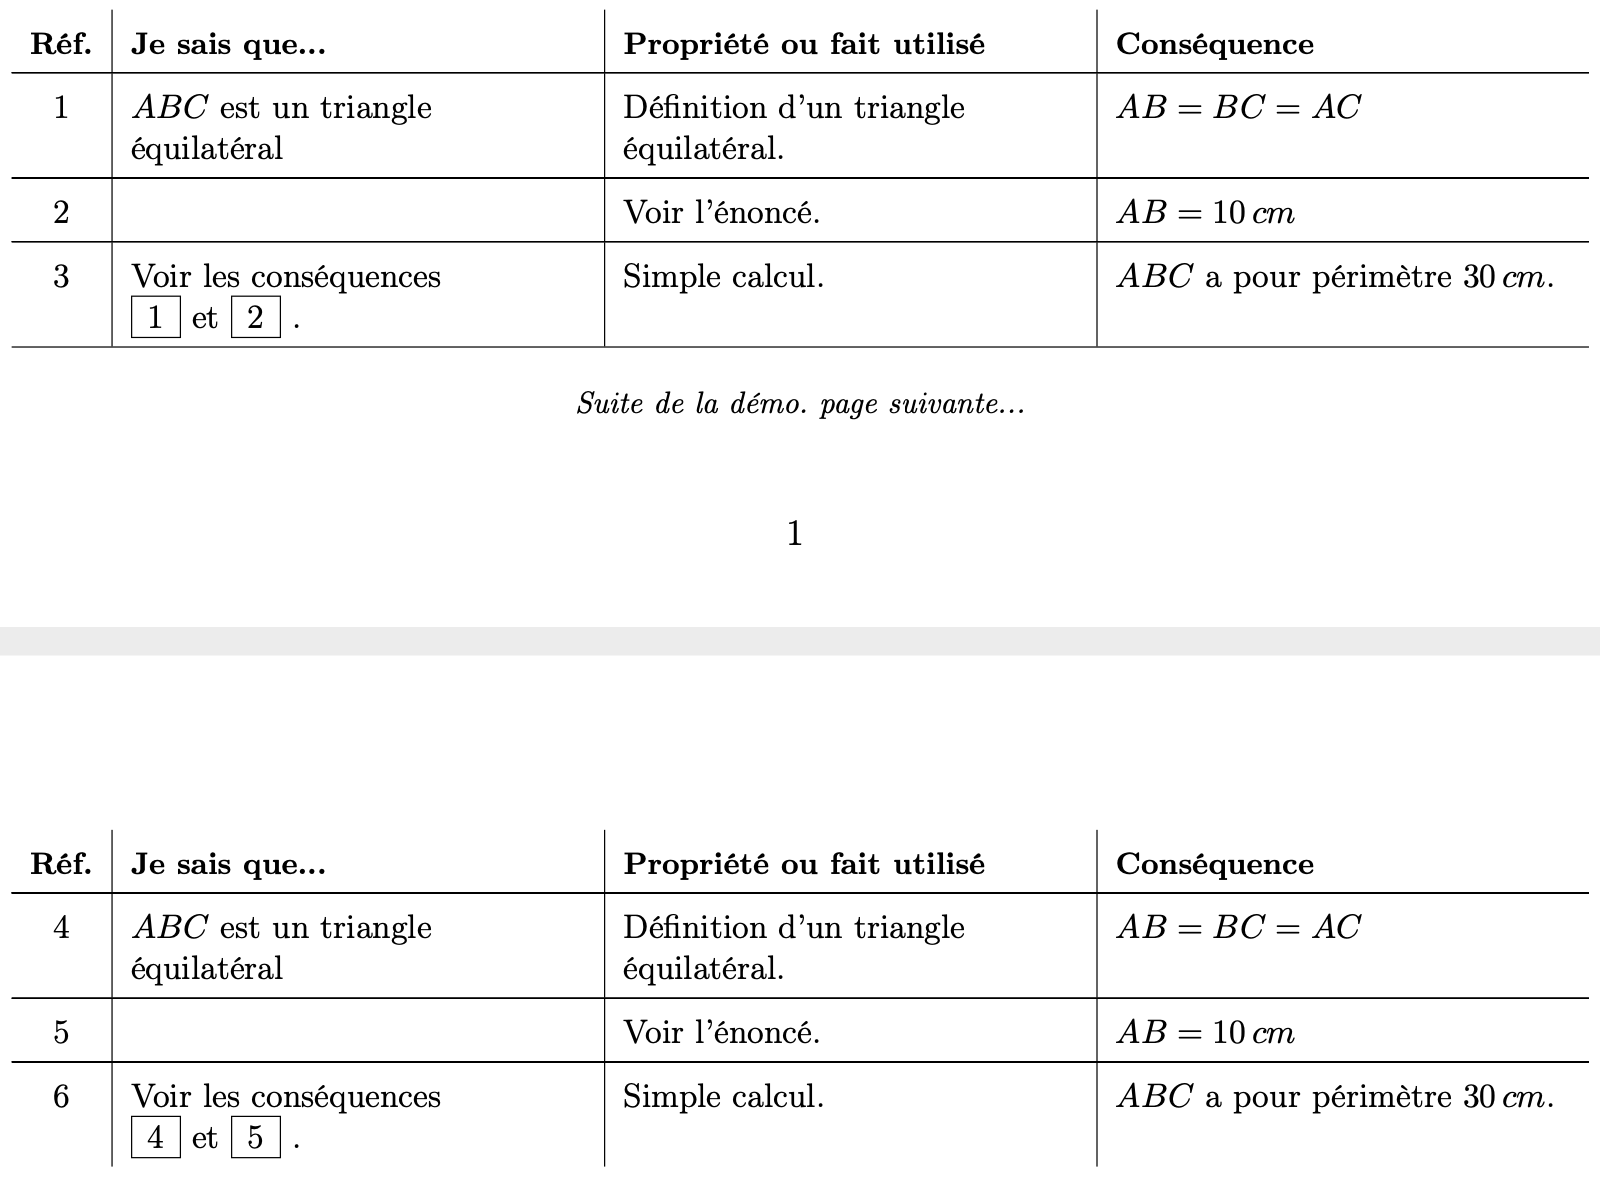
\includegraphics[scale = .5]{images/demo-explained-middleschool-broken[fr].png}}
\end{figure}

\end{document}
